\begin{center}
  \normalsize{\cyr{\textbf{№3.3}}}
\end{center}

\begin{figure}[h!]
  \centering
  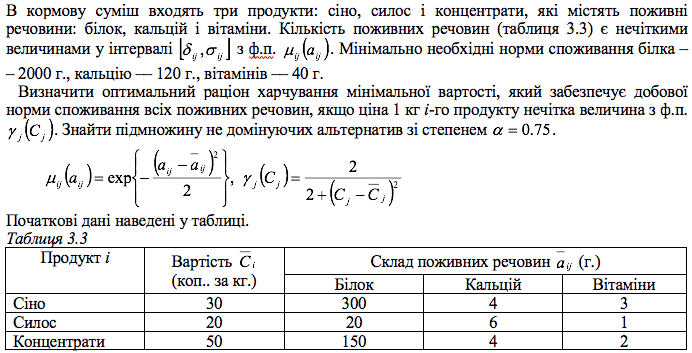
\includegraphics[width=14.1cm]{3_3.png}
  \centering
\end{figure}

Математична модель: $x_{ij}$ вміст поживної речовини  $j$ в продукті $i$
\Code{
min \quad   \sum_i^3\  C_{j} x_{ij} \qquad  \text{Обмеження} \quad  \sum_i^3 a_{ij}  x_{ij} \geqslant b_i
}

\begin{multicols}{2}
  $$\mu(a_{ij}) \geqslant 0.75  $$

  $$ \exp\{ - \dfrac{(a_{ij}-\overline{a}_{ij})^2}{2} \} \geqslant 0.75 $$

  $$- \dfrac{(a_{ij}-\overline{a}_{ij})^2}{2} \geqslant \ln{0.75} $$

  $$ (a_{ij}-\overline{a}_{ij})^2 \leqslant -2 \ln{0.75} $$

  $$ (a_{ij}-\overline{a}_{ij})^2 \leqslant 2 \ln{\dfrac{1}{0.75}} $$


  $$|a_{ij}-\overline{a}_{ij}| \leqslant \sqrt{2\ln{\dfrac{4}{3}}} $$

  $$ \overline{a}_{ij} - \sqrt{2 \ln{\dfrac{4}{3}}} \leqslant a_{ij} \leqslant \overline{a}_{ij} + \sqrt{ 2 \ln{\dfrac{4}{3}}}$$

  \columnbreak
  $$\gamma(C_{i}) \geqslant 0.75 $$

  $$
  \dfrac{2}{2+(C_{j}-\overline{C}_{j})^2} \geqslant 0.75
  $$

  $$
  \dfrac{2}{0.75} \geqslant 2+(C_{j}-\overline{C}_{j})^2
  $$

  $$
  \dfrac{2}{0.75} - 2 \geqslant (C_{j}-\overline{C}_{j})^2
  $$

  $$
  \dfrac{2}{3} \geqslant (C_{j}-\overline{C}_{j})^2
  $$

  $$
  \sqrt{\dfrac{2}{3}} \geqslant |C_{j}-\overline{C}_{j}|
  $$

  $$
  \overline{C}_{j} - \sqrt{\dfrac{2}{3}} \leqslant C_{j} \leqslant \overline{C}_{j} + \sqrt{\dfrac{2}{3}}
  $$

\end{multicols}



\begin{multicols}{2}

  \Title{Задача песиміста}
  \Code{
    min \quad \sum_i^3( \overline{C}_{i} + \sqrt{\dfrac{2}{3}} ) x_{j}
  }

  \Title{Обмеження}
  \Code{
    \sum_j^3( \overline{a}_{ij} + \sqrt{ 2 \ln{\dfrac{4}{3}}} ) x_{j} \geqslant b_i
  }

  \columnbreak

  \Title{Задача оптиміста}
  \Code{
    min \quad \sum_i^3( \overline{C}_{i} - \sqrt{\dfrac{2}{3}} ) x_{j}
  }

  \Title{Обмеження}
  \Code{
    \sum_j^3( \overline{a}_{ij} -  \sqrt{ 2 \ln{\dfrac{4}{3}}}) x_{j} \geqslant b_j
  }

\end{multicols}
